\documentclass[a4paper,12pt]{article}
\usepackage[utf8]{inputenc}
\usepackage[ngerman]{babel}
\usepackage[a4paper, left=2.5cm, right=2.5cm]{geometry}
\usepackage{graphicx}
\usepackage{subcaption}
\usepackage{fancyhdr}
\usepackage{pdfpages}
\usepackage{multirow}
\usepackage{amsmath}
\pagestyle{fancy}
\lhead{Messtechnik Labor}
\chead{}
\rhead{Gruppe 2}

\begin{document}
	%Titelseite
	
\includepdf{LU2_Protokoll_titlepage.pdf}
	
	\noindent
	\textbf{\Large Rechtliches} \\ \\
	Ich bestätige hiermit, dass alle hier verwendeten Messergebnisse und Interpretationen von uns selbst erstellt wurden. Es wurden keine anderen Quellen als die hier schriftlich angegeben verwendet.
	\setcounter{page}{2}
	
	\newpage
	%Inhaltsverzeichnis
	\tableofcontents
	
	\newpage
	\section{Einleitung}
	Die zweite Laborübung beschäftigt sich damit die Charakteristiken unterschiedlicher Impedanzen, mittels gezielter Messungen, zu bestimmen und daraus die Struktur und Bauteilwerte abzuleiten. Zusätzlich beschäftigen wir uns mit der Leistungsmessung mithilfe eines Wattmeters. \\ \newline
	Als Testaufbau dienen fünf Stränge mit unterschiedlichen Impedanzen, welche in einer Blackbox verbaut wurden. Von den Strängen sind die Strukturen bekannt: R, L, C, RL, RC. Die exakten Bauteilwerte sind unbekannt.Die Stränge sind über Anschlussbuchsen von außen zugänglich. \\ \newline
	\begin{figure}[h]
		\centering
		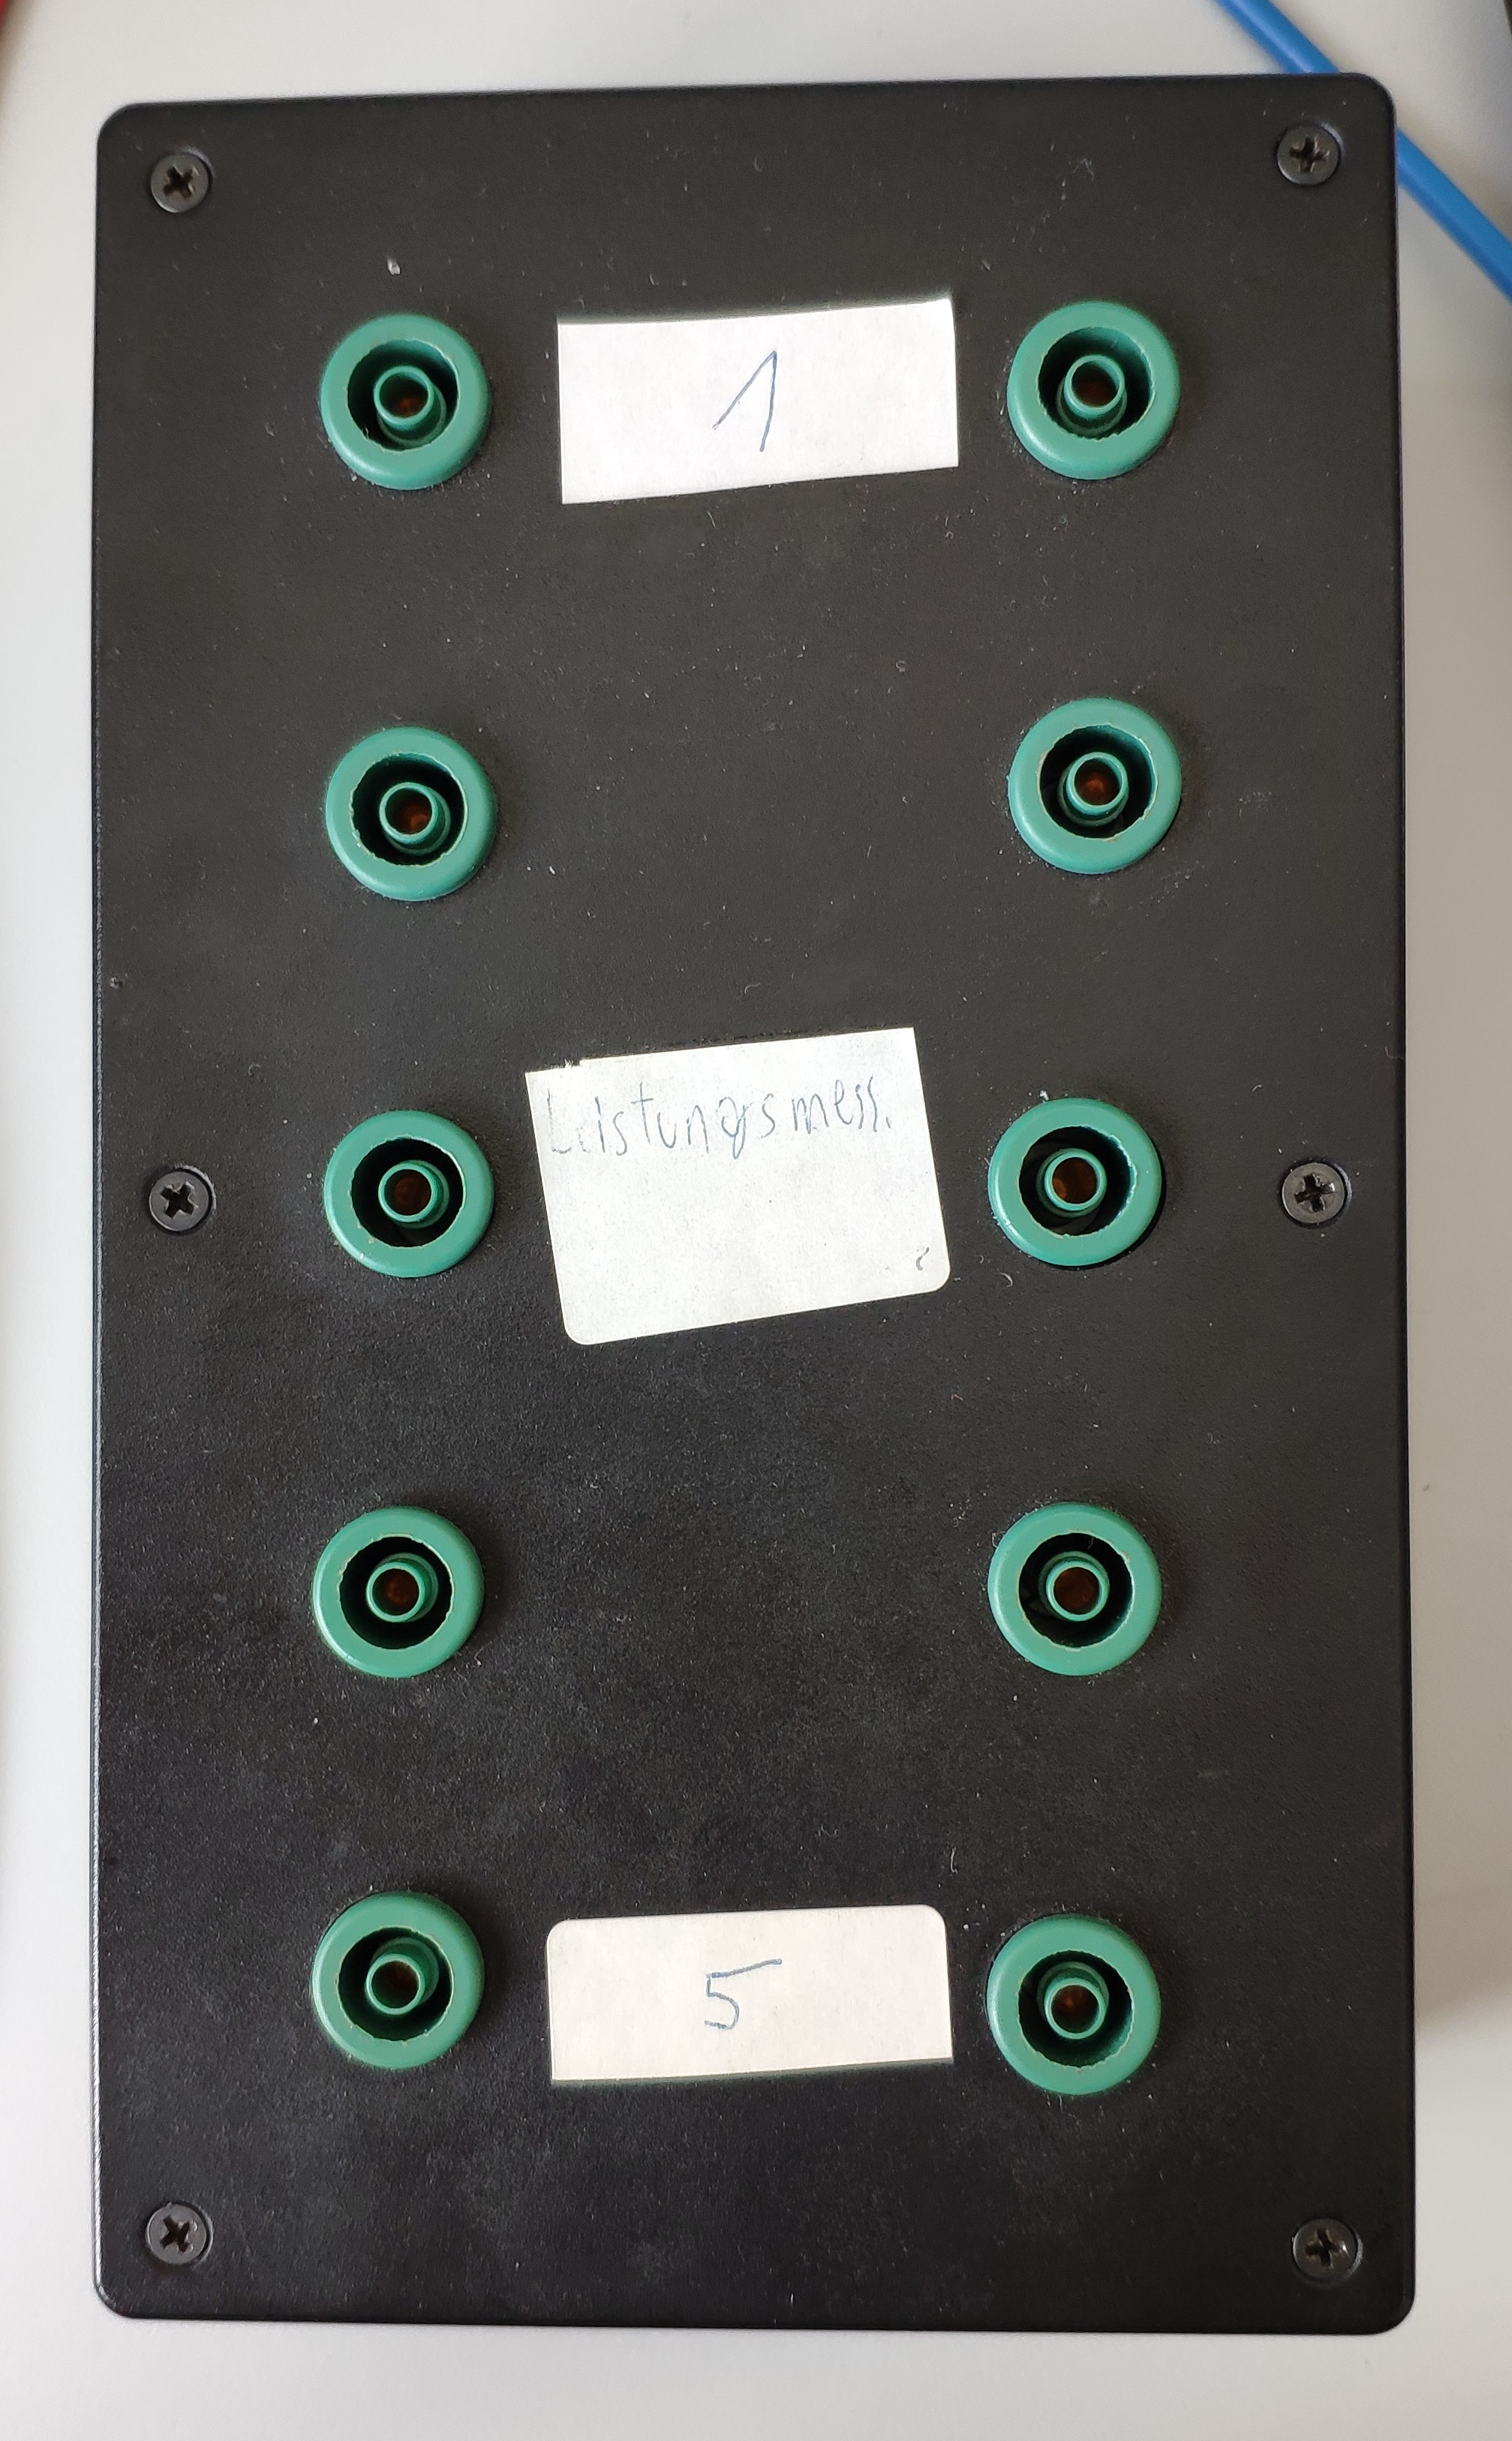
\includegraphics[width=8cm]{assets/blackbox}
		\caption{Blackbox mit unterschiedlichen Impedanzen}
	\end{figure}
	\newline
	Zur Charakterisierung der einzelnen Stränge werden folgende Messungen durchgeführt:
	\begin{itemize}
		\item Strommessung
		\item Widerstandsmessung
		\item Impedanzmessung
		\item Fehlerfortpflanzung
		\item Impedanzmessung mittels LCR-Meter
		\item 5/8-Methode
		\item Leistungsmessung
	\end{itemize}
	\newpage
	\section{Übungsdurchführung}
	\subsection{Strommessung}
	\underline{\textbf{Aufgabenstellung}} \\ \newline
	\noindent
	Für die ersten Aufgabe soll ein der Spannung proportionales Stromsignal am Oszilloskop gemessen werden. Um die Strommessung am Oszilloskop zu ermöglichen, muss der Impedanz-Strang um einen Widerstand, auch Shuntwiderstand genannt, erweitert werden. Aus der Spannung, die am Widerstand abfällt, und dem Widerstandswert kann der Strom, der durch den Strang fließt, errechnet werden.\\
	Aus der zeitlichen Verschiebung zwischen dem Spannungssignal und dem Stromsignal kann die Art der Impedanz abgeleitet werden.
	\\ \newline
	\noindent
	\underline{\textbf{Messaufbau}} \\
	\begin{figure}[h]
		\centering
		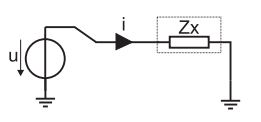
\includegraphics[width=10cm]{assets/strommessung}
		\caption{Schaltung zur Strommessung}
	\end{figure}
	\newline
	Der Messaufbau wird von dem Frequenzgenerator mit einer Spannung versorgt. Es wird ein Sinus-Signal mit \(10V_{pp}\) eingestellt.\\ Damit die Komponenten in der Blackbox nicht beschädigt werden, ist ein maximaler Strom von 5mA vorgeschrieben. Aus diesen Vorgaben ergibt sich für den Shuntwiderstand ein Wert von \[
	R_S = \frac{u_{max}}{i_{max}} = \frac{5V}{5mA} = 1k\Omega
	\]
	\\ \newline
	Somit errechnet sich der Strom, der durch den Strang fließt, zu \[
	i_S = \frac{u_S}{R_S}
	\]
	\newpage
	\subsection{Widerstandsmessung}
	\underline{\textbf{Aufgabenstellung}} \\ \newline
	\noindent
	Damit bei der Bestimmung der Impedanzen Abweichungen des Bauteilwertes bereits in die Berechnungen mit einfließen, wird in dieser Aufgabe zuerst der genaue Wert des Shuntwiderstands bestimmt.\\ Um Messabweichungen einzelner Multimeter zu kompensieren wird der Widerstandswert mit drei unterschiedliche Hand-Multimetern und einem Desktop-Multimeter erfasst.\\ Aus diesen Werten wird im darauf folgenden Schritt der Mittelwert und die Standardabweichung errechnet.\\ \newline
	\noindent
	\underline{\textbf{Messdurchführung mittels Multimeter}}
	\\ \newline
	Zur Messung des Widerstandswertes werden folgende Multimeter genutzt:
	\begin{table}[h]
	\centering
		\begin{tabular}{ll}
			M1 & Agilent U1232A \\
			M2 & Neumann 9140   \\
			M3 & Fluke 87 V     \\
			DM & Agilent 34461A
		\end{tabular}
	\captionof{table}{Multimeter zur Vermessung des Shuntwiderstands}
	\end{table}
	\newline
	Die Auswertung der Messungen ergibt folgende Werte:
	\begin{table}[h]
	\centering
		\begin{tabular}{|c|c|l|}
			\hline
			$Messung$ & $Widerstandswert$ & $Ergebnis$                                                                                    \\ \hline
			M1      & 1077 $\Omega$            & \multirow{4}{*}{\begin{tabular}[c]{@{}l@{}}Mittelwert: 
			\(\displaystyle \bar{R_i}=\frac{1}{4}\sum_{n=1}^4 R_i = 1079.75\Omega\) \\ Standardabweichung: \(\displaystyle s(\bar{R_i})=\sqrt{\frac{\sum_{i=1}^4 (R_i-\bar{R_i})^2}{3}} = 2.2\Omega\)\end{tabular}} \\[2ex] \cline{1-2}
			M2      & 1081 $\Omega$           &                                                                                             \\ \cline{1-2}
			M3      & 1082 $\Omega$           &                                                                                             \\ \cline{1-2}
			DM      & 1079 $\Omega$ &                                                                                             \\ \hline
		\end{tabular}
	\captionof{table}{Auswertung der Widerstands-Vermessung mit unterschiedlichen Multimetern}
	\end{table}
	\newline
	\noindent
	\underline{\textbf{Ermittelung des Mittelwertes und der Standardabweichung}}\\ \newline
	Das Desktop-Multimeter ist in der Lage die Messwerte als Histogramm darzustellen.\\
	Hierzu wurden 5110 Messungen vorgenommen mit einer Aperture von 1 PLC durchgeführt.\\ Die Aperture-Einstellung des Desktop-Multimeters gibt die Dauer einer Messung an. Umso länger eine Messung dauert, umso genauer ist das Ergebnis, da sich der Widerstand nicht so stark erwärmt.\\ \newline
	\begin{figure}[h]
		\centering
		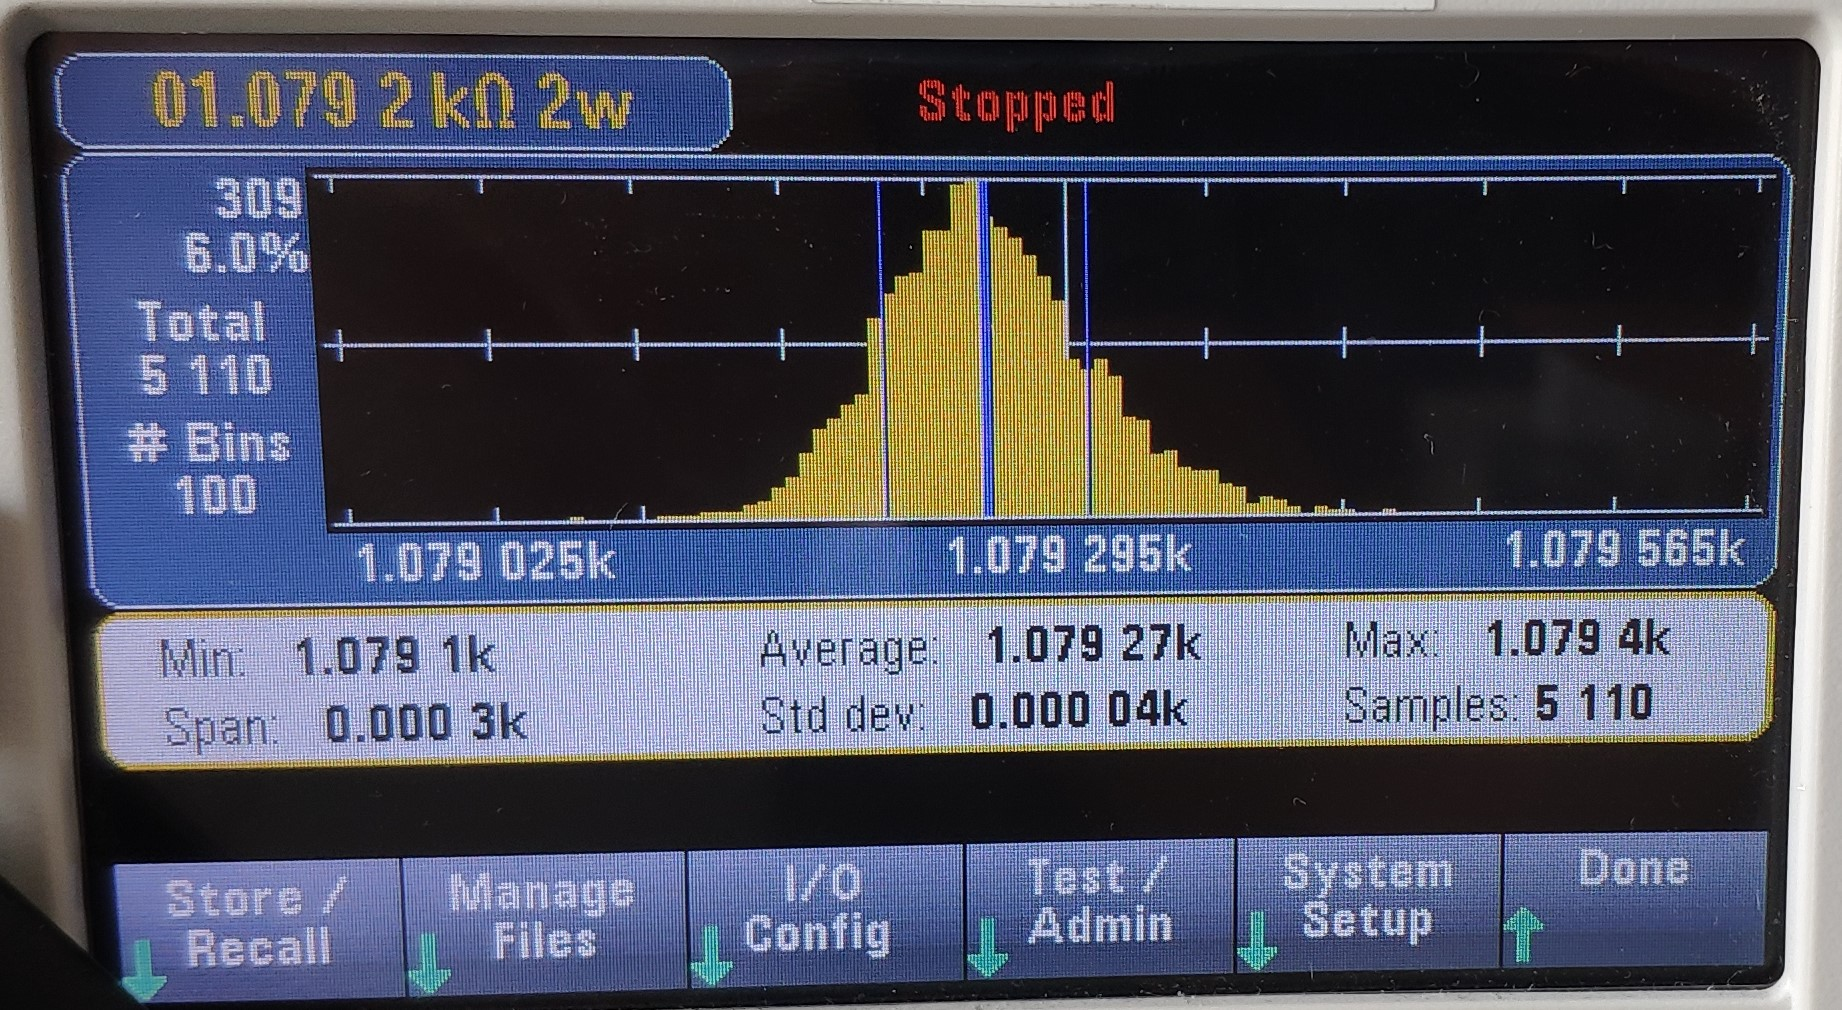
\includegraphics[width=10cm]{assets/digitalmultimeter}
		\caption{Histogramm über 5110 Messungen mit einer Aperture von 1 PLC}
	\end{figure}
	Das Histogramm stellt eine gauß'sche Verteilung dar. Der Mittelwert beträgt 1079.27$\Omega$. Links vom Maximum sind leichte Ausreißer zu erkennen, welche auf die, durch die Messungen, erhöhte Temperatur des Widerstandes zurück zu führen ist.\\ Die Standardabweichung beträgt 40$\mu\Omega$. Die relativ geringe Standardabweichung ergibt sich aus der hohen Anzahl an Messungen, die eine kleine Unsicherheit ermöglichen.\newline
	Zum Vergleich war die Standardabweichung bei einer Aperture von 0.02 PLC mit $200\mu\Omega$ deutlich größer. \newpage
	\subsection{Impedanzmessung}
	\underline{\textbf{Aufgabenstellung}} \\ \newline
	\noindent
	In dieser Aufgabe sollen die Impedanzen, über ihre jeweiligen charakteristischen Eigenschaften, mithilfe eines analogen Oszilloskops bestimmt werden. \\ \newline
	Die Impedanz der Stränge kann aus der zeitlichen Differenz zwischen dem Strom- und Spannungsverlauf abgeleitet werden. Zusätzlich wird die Amplitude des Spannungs- und des Stromsignales gemessen.\\ \newline
	\noindent
	\underline{\textbf{Messaufbau}}
	\\ \newline
	Um den Strom- und den Spannungsverlauf auf dem analogen Oszilloskop darstellen zu können, wird die Schaltung gemäß Abbildung 4 aufgebaut. Als Spannungsversorgung wird ein Siglent SDG1025 verwendet, welches die Schaltung mit einer Sinus-Spannung mit $10V_{pp}$ und einer Frequenz von abwechselnd 1kHz und 15 kHz versorgt. Als Shuntwiderstand wird der in Aufgabe 2.2 vermessene Widerstand genutzt.\\ \newline
	Bei dieser Messung ist es wichtig den Shuntwiderstand hinter der Impedanz direkt auf Masse zu schalten, damit er nicht vom Oszilloskop kurzgeschlossen wird.\newline
	\begin{figure}[h]
		\centering
		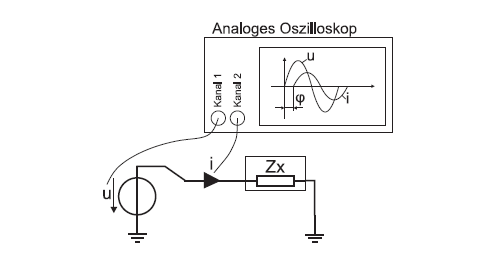
\includegraphics[width=11cm]{assets/impedanzmessung}
		\caption{Messaufbau zur Impedanzmessung}
	\end{figure} \newline
	\noindent
	\underline{\textbf{Strommessung}}\\ \newline
	Am Oszilloskop wird die Spannung über den Shuntwiderstand dargestellt. Aus der Beziehung \(i=\frac{u_R}{\bar{R_i}}\) ergibt sich der Strom zu \(i=\frac{u_R}{1079.75\Omega}\).\\
	\newpage
	\noindent
	\underline{\textbf{Strom- und Spannungsverlauf}}\\ \newline
	Durch Aktivieren der Spannungsversorgung lässt sich am Oszilloskop ein Bild, wie in Abbildung 5, erkennen. \newline
	\begin{figure}[h]
		\centering
		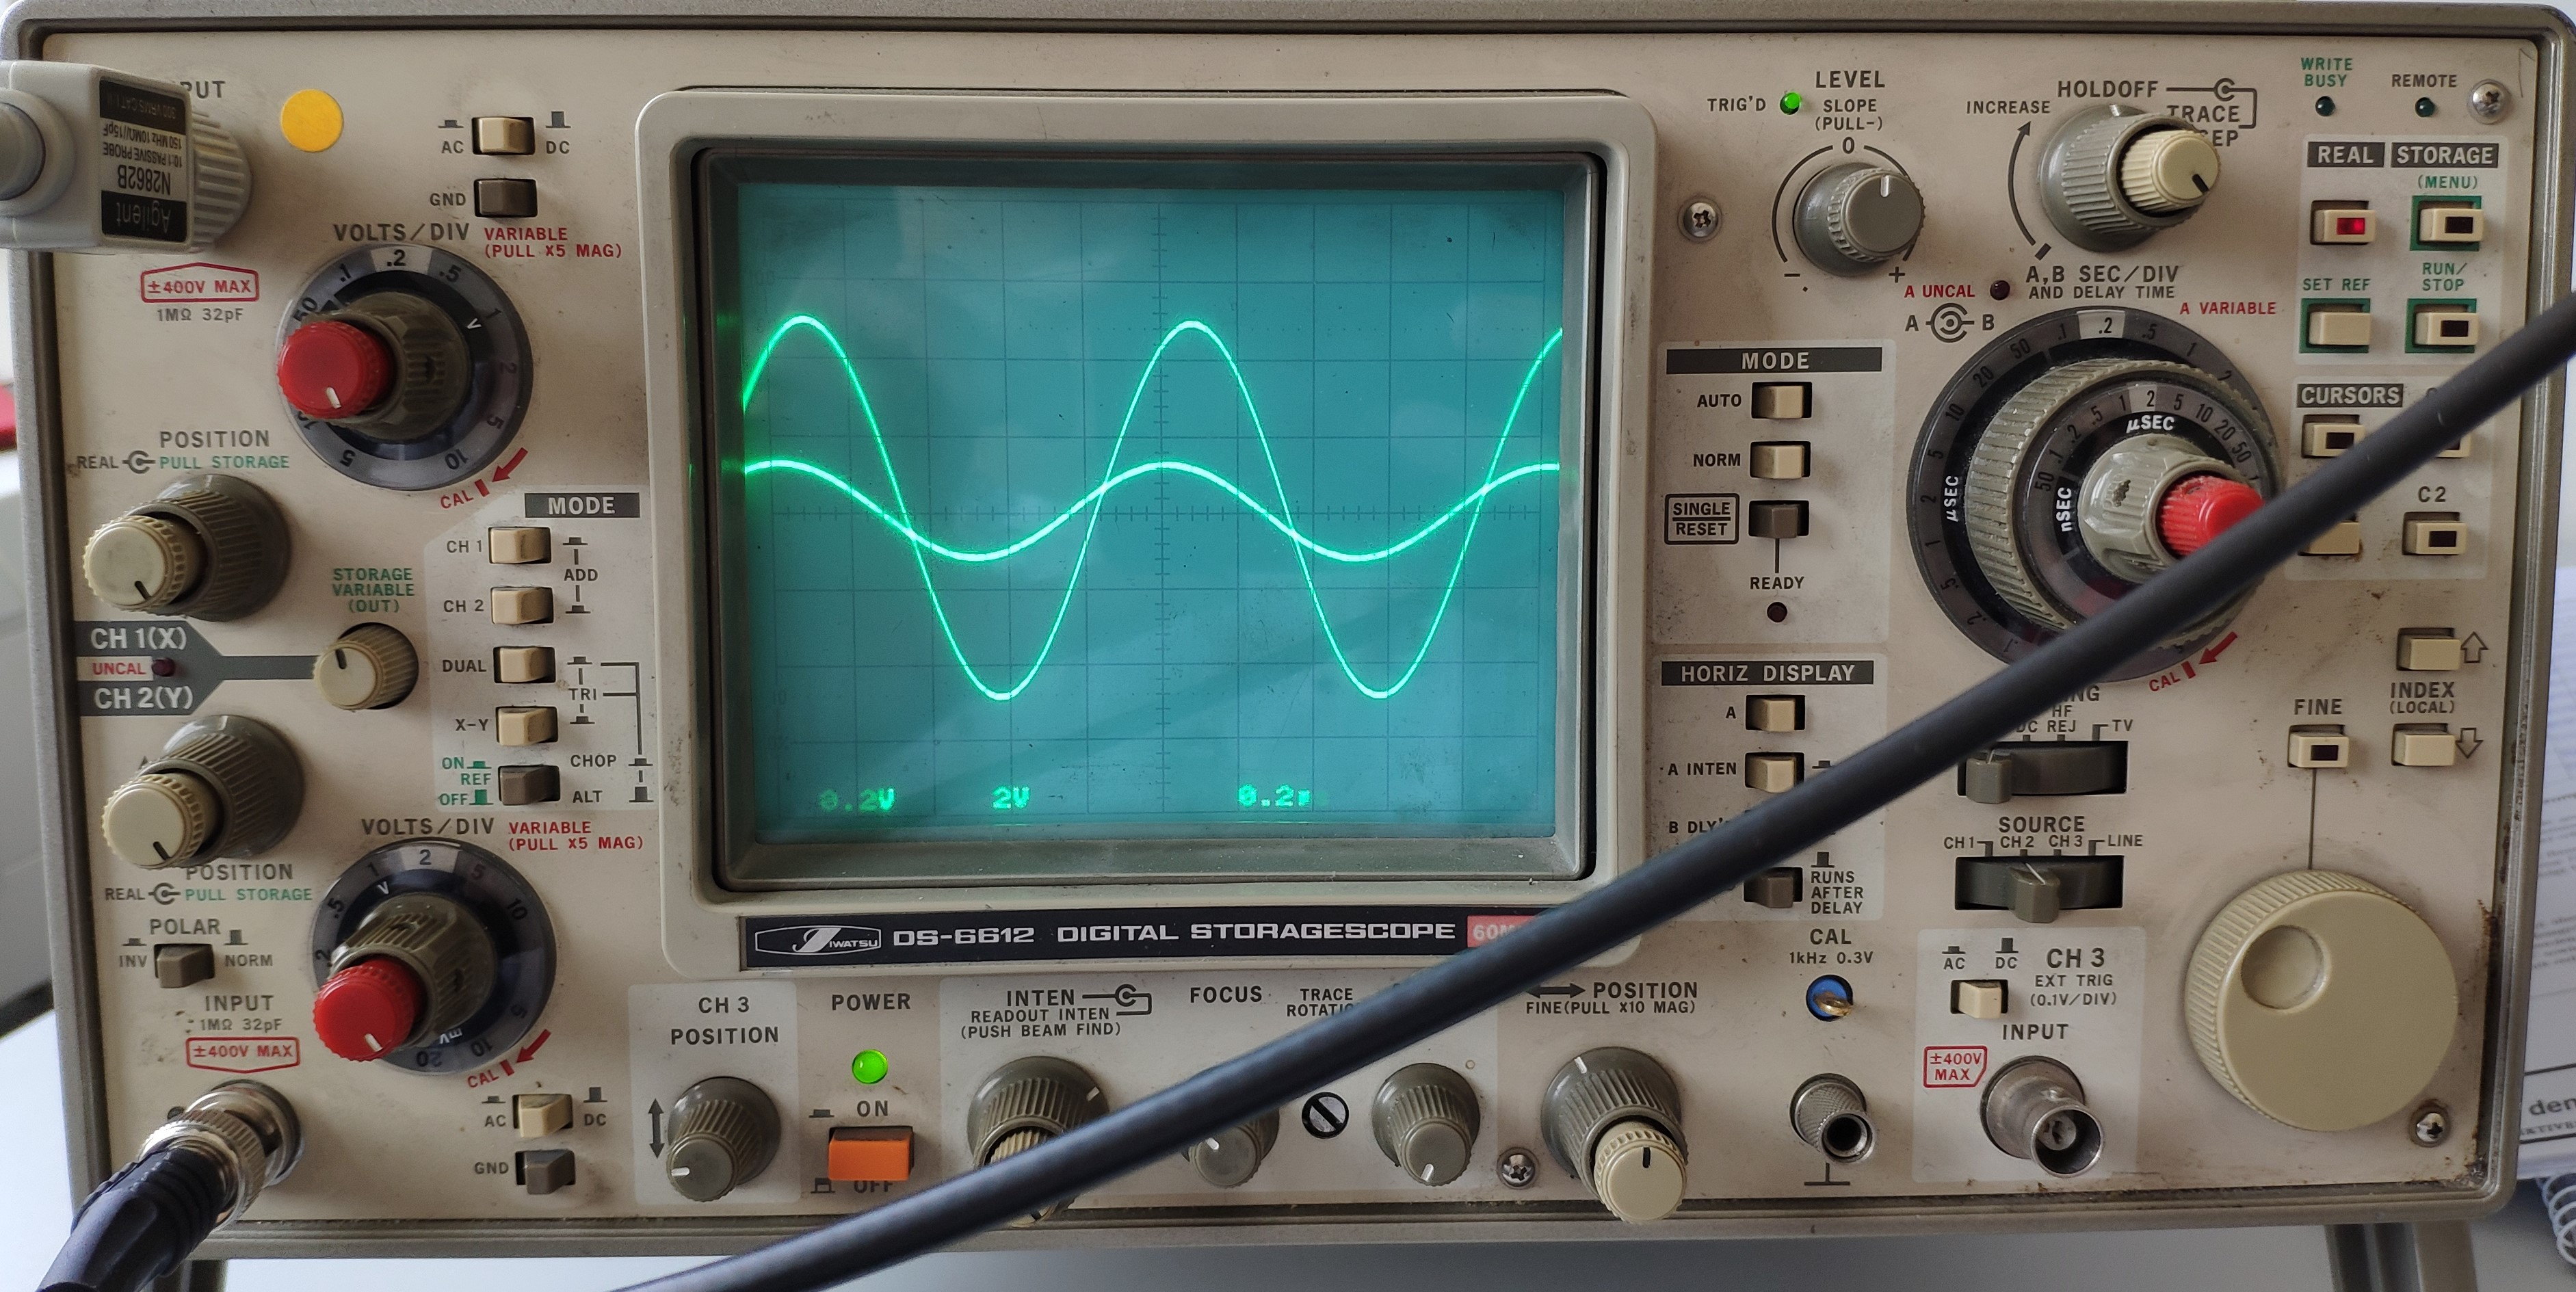
\includegraphics[width=11cm]{assets/strom_spannung}
		\caption{Strom- und Spannungsverlauf am analogen Oszilloskop}
	\end{figure}
	\newline
	Nun kann am Oszilloskop die zeitliche Verschiebung zwischen der Spannung und dem Strom gemessen werden.\\ Mithilfe der zeitlichen Differenz kann der Phasenwinkel aus \(\frac{\Delta t}{T}=\frac{\Delta \Phi}{360\circ}\) errechnet werden. Die Periodendauer ergibt sich zu \(T=\frac{1}{f}\). \\ \newline
	Daraus kann die Impedanz errechnet werden.
	\[Z=|Z|e^{j\Phi}=\frac{u}{i}\cos(\Phi) + j \sin(\Phi)\]\newpage
	\begin{table}[h]
	\centering
		\begin{tabular}{|c|c|c|c|c|c|}
			\hline
			\multicolumn{1}{|l|}{$Strang$} & \multicolumn{1}{l|}{$f [kHz]$} & \multicolumn{1}{l|}{$u [V]$} & \multicolumn{1}{l|}{$i [A]$} & \multicolumn{1}{c|}{$Z[\Omega]$} & $Struktur$ \\ \hline
			\multirow{2}{*}{S1}            & 1                              & 5                            & 1.2m                         & 2651.27 - j 2007.30              & RC         \\ \cline{2-6} 
			& 15                             & 5                            & 1.6m                         & 2125 - j 0                       & RC         \\ \hline
			\multirow{2}{*}{S2}            & 1                              & 5                            & 2.6m                         & 30.44 - j 1623.71                & RC         \\ \cline{2-6} 
			& 15                             & 5                            & 4m                           & 250 - j 0                        & RC         \\ \hline
			\multirow{2}{*}{S3}            & 1                              & 5                            & 4m                           & 250 + j 0                        & RL         \\ \cline{2-6} 
			& 15                             & 5                            & 4m                           & 162.22 + j 460.55                & RL         \\ \hline
			\multirow{2}{*}{S4}            & 1                              & 5                            & 4m                           & 210.72 + j 310.86                & RL         \\ \cline{2-6} 
			& 15                             & 5                            & 1.2m                         & 36.2 + j 4035.76                 & RL         \\ \hline
			\multirow{2}{*}{S5}            & 1                              & 5                            & 3m                           & 666.67 + j 0                     & R          \\ \cline{2-6} 
			& 15                             & 5                            & 2.5m                         & 1000 + j 0                       & R          \\ \hline
		\end{tabular}
	\captionof{table}{Berechnung der Impedanzen und Ermittelung der Struktur}
	\end{table}
	\noindent
	\underline{\textbf{Ermittelung der Impedanz-Struktur}}\\ \newline
	Für den Strom- und Spannungsverlauf über Impedanzen gilt:\newline
	Eilt der Strom der Spannung voraus, handelt es sich bei dem Strang um eine kapazitive Last (ein reines C- oder RC-Glied). In diesem Fall ist der Phasenwinkel negativ.\newline Wenn jedoch die Spannung dem Strom voraus eilt, handelt es sich bei dem Strang um eine induktive Last (ein reines L- oder RL-Glied). Der Phasenwinkel ist dann positiv.\\ \newline
	\begin{itemize}
		\item S1 - Im ersten Strang ist ein negativer Phasenwinkel zu erkennen was auf ein kapazitives Verhalten schließen lässt. Da die reale Impedanz $2.65k\Omega$ beträgt, wobei $1k\Omega$ von unserem Shuntwiderstand kommen, muss es sich bei diesem Strang um einen \(RC\) Strang handeln. 
		$R = 1.65k\Omega , C = 79.28nF$
		\item S2 - In diesem Strang ist ebenfalls ein negativer Phasenwinkel zu erkennen, was wieder auf ein kapazitives Verhalten schließe lässt. Da von unserem Shuntwiderstand $1k\Omega$ in die Berechnung mit einfließt, beträgt die übrige reale Impedanz des Stranges nur $30\Omega$, was vom Innenwiderstand eines Kondensators kommen kann. Daher muss es sich bei diesem Strang um einen reines \(C\)-Glied handeln. $C = 98.01nF$
		\item S3 - Im dritten Strang ist ein positiver Phasenwinkel zu erkennen, was auf eine induktive Last hindeutet. Da in diesem Fall der reale Teil der Impedanz mit $250\Omega$ relativ groß ist, ist es unwahrscheinlich, dass er vom Innenwiderstand der Spule kommt. Somit handelt es sich in diesem Fall um einen \(RL\) Strang. \\$R = 250\Omega , L = 4.88mH$
		\newpage
		\item S4 - Im vierten Strang eilt ebenfalls die Spannung dem Strom voraus. Wir gehen daher auch in diesem Fall von einem induktiven Glied aus. Da die reale Impedanz mit $36\Omega$ relativ gering ist, kann man hier von einem reinen \(L\) Strang ausgehen. \\
		$L = 49.47mH$
		\item S5 - Im fünften Strang ist keine zeitliche Verschiebung zwischen dem Strom und der Spannung zu erkennen. Wir gehen daher von einem reinen \(R\) Glied aus. $R = 1000\Omega$
	\end{itemize}
	\newpage
	\subsection{Fehlerfortpflanzung}
	\underline{\textbf{Aufgabenstellung}} \\ \newline
	\noindent
	Ziel dieser Aufgabe ist es die gesamte Unsicherheit der Wirkleistung am RL-Strang (in unserem Fall Strang 3) zu berechnen. Hierzu sind die Messung der Spannung, des Stroms und des Phasenwinkels erforderlich. \\ \newline
	\noindent
	\underline{\textbf{Messaufbau}}
	\\ \newline
	Um die Messung von Spannung, Strom und Phasenwinkel durchzuführen, wird die Schaltung wie in Abbildung 4 aufgebaut.\newline In dieser Aufgabe ersetzen wir jedoch das analoge durch das digitale Oszilloskop, da es uns die schnelle Berechnung der RMS-Werte von Spannung und Strom ermöglicht.\\ \newline
	Am Funktionsgenerator wird ein Sinus-Signal mit $10V_{pp}$ und einer Frequenz von $150Hz$ eingestellt.\\ \newline
	\noindent
	\underline{\textbf{Berechnung von Wirkleistung, Mittelwert und Standardabweichung}}\\ \newline
	Die Formel zur Berechnung der Wirkleistung lautet \[
	P = U I \cos(\Phi)
	\]\\ \newline
	Die Berechnung des Mittelwerts erfolgt aus 
	\[\displaystyle \bar{P}=\frac{1}{N}\sum_{n=1}^N P_i \] \\ \newline
	Die Standardabweichung errechnet sich zu \[\displaystyle s(\bar{P})=\sqrt{\frac{\sum_{i=1}^N (P_i-\bar{P})^2}{N-1}} \]
	In dieser Aufgabe sollten fünf unterschiedliche Werte für den Strom und den Phasenwinkel gemessen werden.\newline Um Abweichungen zwischen den Werten zu erhalten, wurde am Oszilloskop mithilfe unterschiedlicher Measure-Funktionen eine gewollte Abweichung zwischen den Messungen erzeugt.\\ \newline
	\begin{table}[h]
	\centering
		\begin{tabular}{|c|c|c|}
			\hline
			$Messung Nr.$ & $x_1 = I_{RMS} [A]$ & $x_2 = \Phi[rad]$\\ \hline
			\multicolumn{1}{|c|}{1} & \multicolumn{1}{c|}{3.57m} & \multicolumn{1}{c|}{0.052} \\ \hline
			\multicolumn{1}{|c|}{2} & \multicolumn{1}{c|}{3.36m}  & \multicolumn{1}{c|}{0.0634} \\ \hline
			\multicolumn{1}{|c|}{3} & \multicolumn{1}{c|}{3.579m} & \multicolumn{1}{c|}{0.049} \\ \hline
			\multicolumn{1}{|c|}{4} & \multicolumn{1}{c|}{3.39m}  & \multicolumn{1}{c|}{0.0536} \\ \hline
			\multicolumn{1}{|c|}{5} & \multicolumn{1}{c|}{3.67m}  & \multicolumn{1}{c|}{0.0572} \\ \hline
			$\bar{x_i}$ & 3.51m & 55m \\ \hline
			$s(\bar{x_i})$ & $133\mu$ & 5.516m \\ \hline
			$\frac{\partial P}{\partial x_i}$ & 3.53 & -0.967m \\ \hline
			$(\frac{\partial P}{\partial x_i})^2 s^2(\bar{x_i})$ & 221n & 93n \\ \hline
			Kovarianz  & \multicolumn{2}{c|}{-$0.329\mu$} \\ \hline
			$s(\bar{P})$ & \multicolumn{2}{c|}{0.56m}\\ \hline
		\end{tabular}
	\captionof{table}{Strom und Phasenwinkel Messung}
	\end{table}\newline
	\textbf{Verwendete Formeln:}
	\begin{align*}
		&\text{Mittelwert:} \ \bar{x} = \frac{1}{N} \sum_{i=1}^{N}x_i \\
		&\text{Standardabweichung:} \ s(\bar{x}_i) = \sqrt{\frac{1}{N-1}\sum_{i=1}^{N}(x_i - \bar{x}_i)^2} \\
		&\text{Kovarianz:} \ cov(x_1,x_2) = \frac{1}{N-1} \sum_{i=1}^{N}(x_{1i} - \bar{x}_{1i})(x_{2i} - \bar{x}_{2i})  \\
		&s(\bar{P}) = \left(\frac{\partial P}{\partial x_1}\right)^2 s^2(\bar{x}_1) + \left(\frac{\partial P}{\partial x_2}\right)^2 s^2(\bar{x}_2) + \frac{\partial P}{\partial x_1}\frac{\partial P}{\partial x_2}cov(x_1,x_2)
	\end{align*}
	\newpage
	\subsection{Impedanzmessung mittels LCR-Meter}
	\underline{\textbf{Aufgabenstellung}} \\ \newline
	\noindent
	Die Aufgabe hat als Ziel die Ergebnisse der Impedanz-Berechnung zu bestätigen. Hierzu wird im Labor ein Philips PM 6303 LCR-Meter zur Verfügung gestellt. \\ \newline
	\noindent
	\underline{\textbf{Impedanzmessung mittels LCR-Meter}}
	Mithilfe eines LCR-Meters ist möglich die Impedanz in einem Strang in seine Bestandteile aufzuteilen. Das LCR-Meter zeigt nämlich nicht nur die Gesamtimpedanz an, sondern kann die Impedanz auch in die einzelnen Komponenten, also R, C und L, aufteilen.\\ \newline Zur Messung wird eine Frequenz von 1kHz eingestellt. Über die Pfeiltasten kann zwischen $R_s$, $C_s$ und $L_s$ gewechselt werden. In den unterschiedlichen Modi misst das LCR-Meter dann den Real- bzw. den Imaginär-Teil der Impedanz.\\ \newline
	Der Serienwiderstand ist für diese Messung nicht mehr erforderlich. \newline
	\begin{table}[h]
	\centering
		\begin{tabular}{|c|c|c|c|}
			\hline
			\multicolumn{1}{|l|}{$Strang$} & \multicolumn{1}{l|}{C/L [F/H]} & \multicolumn{1}{l|}{$R [\Omega]$} & \multicolumn{1}{l|}{$Z [\Omega]$} \\ \hline
			S1                             & 99.54nF                            & 2.689k                                             & 3.129k                                             \\ \hline
			S2                             & 94.05nF                            & 36.25                                              & 1.693k                                             \\ \hline
			S3                             & 1.182mH                            & 17.9                                               & 19.42                                              \\ \hline
			S4                             & 54.19mH                            & 15.92                                              & 340.9                                              \\ \hline
			S5                             & /                                  & 986.7                                              & 986.7                                              \\ \hline
		\end{tabular}
	\captionof{table}{Auswertung der Messung mittels LCR-Meter}
	\end{table}\newline
	\newpage
	\subsection{5/8-Methode}
	\underline{\textbf{Aufgabenstellung}} \\ \newline
	\noindent
	Ziel dieser Aufgabe ist es die Induktivität des L-Stranges (in unserem Fall Strang 4) zu bestimmen. Hierzu wird die 5/8-Methode benutzt, mit welcher der Wert von $\tau$ bestimmt werden kann. Unter dem Wissen der Widerstandswerte des Shuntwiderstands und des Innenwiderstands der Spule kann daraus die Induktivität errechnet werden.\\ \newline
	\noindent
	\underline{\textbf{Messaufbau}}\\ \newline
	Der Messaufbau, für die 5/8-Methode, erfolgt wie in Abbildung 6 dargestellt.
	\begin{figure}[h]
		\centering
		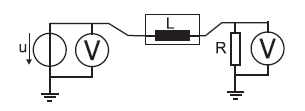
\includegraphics[width=8.1cm]{assets/58methode}
		\caption{Messaufbau zur Bestimmung von L anhand der 5/8-Methode}
	\end{figure}\newline
	\noindent
	\underline{\textbf{Darstellen eines Einschwingvorgangs}}\\ \newline
	Als Eingangsspannung wird ein Rechtecksignal mit einer geringen Frequenz angelegt.\newline Mithilfe der Single-Shot Funktion des Oszilloskops kann ein Einschwingvorgang am Bildschirm dargestellt werden.
	\begin{figure}[h]
		\centering
		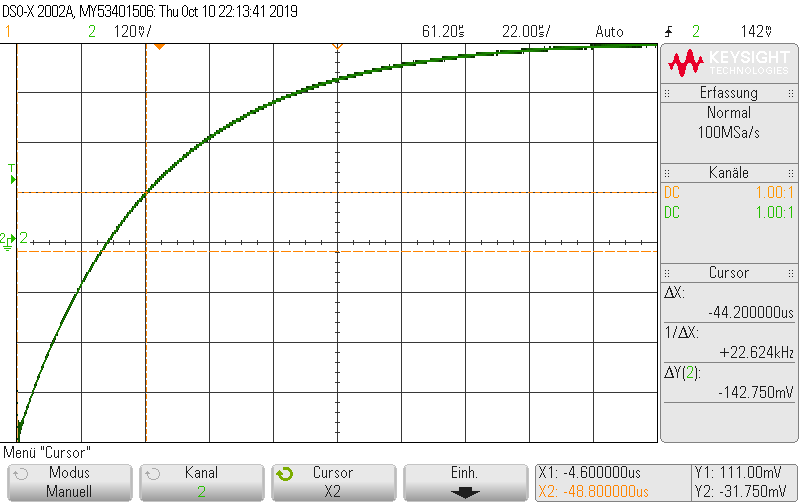
\includegraphics[width=10cm]{assets/58methode_oszi}
		\caption{Der Einschwingvorgang des L-Strangs}
	\end{figure}\newline
	Bei der 5/8-Methode wird das Oszilloskop so eingestellt, dass das Signal durch die linke untere Ecke läuft und der stationäre Endwert am oberen Bildschirmrand ausgerichtet ist.
	Beim Schnittpunkt der 5. vertikalen Unterteilung mit unserer aufgenommenen Kurve, hat das Signal circa 62.5\% (5/8-tel) des Endwertes erreicht.\newline
	Die Zeitdifferenz zwischen dem linken Bildschirmrand und dem oben beschriebene Schnittpunkt entspricht der Zeitkonstante $\tau$.\newline In unserem Fall entspricht das $\tau$ = $45.2\mu s$.\newline
	\newpage
	\noindent
	\underline{\textbf{Berechnung der Induktivität}}\\ \newline
	Aus der Formel \[
	\tau = \frac{L}{R}
	\] lässt sich die Induktivität bestimmen.\\ \newline
	Da sich die Widerstände im Fall einer realen Spule aus $R$ und $R_L$ (dem Innenwiderstand der Spule) zusammensetzen, folgt
	\[
		L = \tau(R + R_L) = 44.2\mu s(1079.75\Omega + 15.92\Omega) = 49.52mH
	\]Der Innenwiderstand der Spule kann aus der Tabelle 5 abgelesen werden.\newline Die Abweichung von ungefähr $5mH$ ist durch Ungenauigkeiten beim Ablesen vom Oszilloskop zu erklären.
	\begin{table}[h]
		\centering
		\begin{tabular}{|c|c|}
			\hline
			\multicolumn{1}{|c|}{\multirow{2}{*}{}} & \multirow{2}{*}{\textbf{L[mH]}} \\
			\multicolumn{1}{|c|}{} &  \\ \hline
			\multirow{2}{*}{\textbf{Oszilloskop}} & \multirow{2}{*}{$49.47$} \\
			&  \\ \hline
			\multirow{2}{*}{\textbf{LCR-Meter}} & \multirow{2}{*}{$54.19$} \\
			&  \\ \hline
			\multirow{2}{*}{\textbf{$5/8$ - Methode}} & \multirow{2}{*}{$49.52$} \\
			&  \\ \hline
		\end{tabular}
		\caption{Vergleich der unterschiedlichen Messarten von Strang 4}
	\end{table}
	\newpage
	\subsection{Leistungsmessung}
	\underline{\textbf{Aufgabenstellung}} \\ \newline
	\noindent
	Ziel dieser Aufgabe ist es mithilfe eines Wattmeters die Leistung des RL-Strangs (in unserem Fall Strang 3) zu messen.\\ \newline
	\noindent
	\underline{\textbf{Messaufbau}}\\ \newline
	Zur Leistungsmessung wird ein Rohde \& Schwarz Hameg Wattmeter genutzt.
	Um den Frequenzgenerator bei der Messung vor der Belastung zu schützen, wird ein Impedanzwandler, wie in Abbildung 8, zwischengeschaltet.\\ \newline
	\begin{figure}[h]
		\centering
		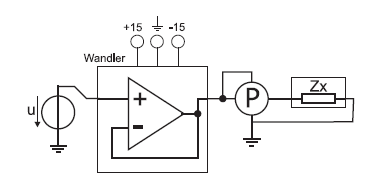
\includegraphics[width=10cm]{assets/leistungsmessung}
		\caption{Schaltung zur Leistungsmessung mit einem Wattmeter}
	\end{figure} \\ \newline
	Der Impedanzwandler wird mit einer bipolaren Spannung von $+-15V$ und einer Strombegrenzung von $300mA$ versorgt. Am Frequenzgenerator wird ein Sinus-Signal mit $7 V_{pp}$ und $100Hz$ eingestellt.\\ \newline
	\noindent
	\underline{\textbf{Leistungsmessung mittels Wattmeter}}\\ \newline
	Nun können am Wattmeter die Scheinleistung, Wirkleistung und Blindleistung abgelesen werden.\newline
	Bei unserer Messung ergab sich durch die begrenzte Genauigkeit des Wattmeters ein Messfehler. Dieser Messfehler macht sich dadurch ersichtlich, dass die Scheinleistung geringer ist, als die Summe der Blindleistung und der Wirkleistung.\newline Das ist dadurch zu begründen, dass das Wattmeter nur eine Auflösung von fünf Digits bietet.\newline
	\begin{table}[h]
	\centering
		\begin{tabular}{|c|c|}
			\hline
			Scheinleistung $[VA]$ & 0.311 \\ \hline
			Wirkleistung $[W]$    & 0.312 \\ \hline
			Blindleistung $[Var]$ & 0.02  \\ \hline
			Leistungsfaktor         & 1     \\ \hline
		\end{tabular}
	\captionof{table}{Auswertung der Messung mittels Wattmeter}
	\end{table}\newline
	\begin{figure}[h]
		\centering
		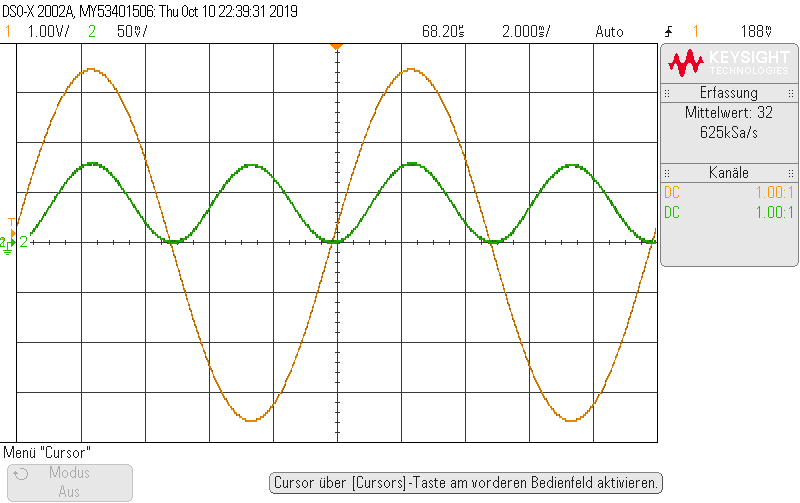
\includegraphics[width=10cm]{assets/momentan-leistung}
		\caption{Darstellung der Momentan-Leistung am Oszilloskop (grün)}
	\end{figure} \\ \newline
	Durch die Messung der Spannung, des Stroms und des Phasenwinkels konnten wir die Leistung zusätzlich berechnen.\newline
	\begin{table}[h]
	\centering
		\begin{tabular}{|c|c|}
			\hline
			Scheinleistung $[VA]$ & 0.315 \\ \hline
			Wirkleistung $[W]$    & 0.314 \\ \hline
			Blindleistung $[Var]$ & 0.05  \\ \hline
			Leistungsfaktor         & 0.99914     \\ \hline
		\end{tabular}
		\captionof{table}{Berechnung der Leistung aus Spannung, Strom und Phasenwinkel}
	\end{table}
	\newpage
	\noindent
	\textbf{Interpretation:} \\ \\
	Die Frequnez der Momentanleistung (grün) schwingt mit der doppelten Frequenz, was auch zu erwarten war. Da es sich hier eigentlich um eine induktive Last handelt, sollte eigentlich eine Phasenverschiebung erkennbar sein, diese tritt aber nicht auf. Dies folgt daraus das die Induktivität so einen geringen Wert hat, sodass dieser die Phase kaum um einen veränderbaren Wert dreht.\\
	Die doppelte Frequenz beruht darauf:
	\begin{align*}
		p = ui &= 2UI\cos(\omega t + \varphi_u)\cos(\omega t + \varphi_i) \\
			   &= UI\cos(\varphi) + UI\cos(2\omega t + \varphi_u + \varphi_i) \\
			   &= P + S\cos(2\omega t + \varphi_u + \varphi_i) \\
		\varphi &= \varphi_u - \varphi_i
	\end{align*}
	Der Mittelwert des in Abbildung 9 zu sehenden Signales (grün) ist die Wirkleistung P. Die Amplituden der Schwingung, die um P mit der doppelten Frequenz schwingt, ist die Scheinleistung S.
	\section{Verwendete Geräte}
	\begin{itemize}
		\item Blackbox 1
		\item Agilent U1232A - Hand-Multimeter
		\item Neumann 9140 - Hand-Multimeter
		\item Fluke 87 V - Hand-Multimeter
		\item Agilent 34461A - Desktop-Multimeter
		\item Rigol DP832 - Spannungsversorgung
		\item Rohde\&Schwarz Hameg - Wattmeter
		\item Philips PM 6303 - RCL-Meter
		\item DS-6612 Digital Storagescope - Analoges Oszilloskop
		\item Agilent DSO-X 2002A - Digitales Oszilloskop
	\end{itemize}
	\newpage
	\listoffigures
	\newpage
	\newpage
	\listoftables
	\newpage
\end{document}